\usepackage{amsthm}

\newtheorem{theorem}{Theorem}[chapter]
\newtheorem{lemma}           [theorem] {Lemma}   
\newtheorem{folg}           [theorem] {Folgerung}   

\newtheorem{frage}       [theorem] {Frage}   
\newtheorem{question}       [theorem] {Question}   
\newtheorem{aufgabe}       [theorem] {Aufgabe}   
\newtheorem{exercise}       [theorem] {Exercise}  

\newtheorem{proposition}     [theorem] {Proposition}  
\newtheorem{satz}     [theorem] {Satz}  
\newtheorem{fact}{Fact}
\newtheorem{definition}      [theorem] {Definition} 

\theoremstyle{definition} 
\newtheorem{bemerkung}     [theorem] {Bemerkung}  
\newtheorem{beispiel}       [theorem] {Beispiel}  
\newtheorem{example}       [theorem] {Example}  
\newtheorem*{example*} {Example}  
\newtheorem{notation}       [theorem] {Notation}  
\newtheorem*{Faust}[theorem]{Rule of Thumb}
\newtheorem*{Boxx}[theorem]{Concept}

\begin{Definition}[Subsequence]
Let $(a_n)_{n\in\mathbb{N}}$ be a~sequence in $\mathbb{K}$. Let $(n_k)_{k\in\mathbb{N}}$ be a~strongly monotonically increasing sequence with $n_k\in\mathbb{N}$ for all $k\in\mathbb{N}$. Then
$(a_{n_k})_{k\in\mathbb{N}}$ is called a~{\em subsequence}.
\end{Definition}

\begin{center}
  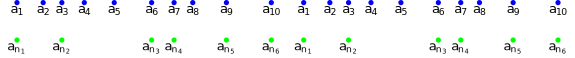
\includegraphics{./107-tikz.svg}
\end{center}

\begin{example}
Consider the sequence $(a_n)_{n\in\mathbb{N}}=(\frac1n)_{n\in\mathbb{N}}$. Then some subsequences are given by
\begin{itemize}
 \item $(a_{n_k})_{k\in\mathbb{N}}=(a_{2k})_{k\in\mathbb{N}}=(\frac12,\frac14,\frac16,\frac18,\ldots)$;
 \item $(a_{n_k})_{k\in\mathbb{N}}=(a_{k^2})_{k\in\mathbb{N}}=(1,\frac14,\frac19,\frac1{16},\frac1{25},\ldots)$;
 \item $(a_{n_k})_{k\in\mathbb{N}}=(a_{2^k})_{k\in\mathbb{N}}=(\frac12,\frac14,\frac18,\frac1{16},\frac1{32},\ldots)$;
 \item $(a_{n_k})_{k\in\mathbb{N}}=(a_{k!})_{k\in\mathbb{N}}=(1,\frac12,\frac16,\frac1{24},\frac1{120},\frac1{720},\ldots)$.
\end{itemize}
\end{example}

\begin{Theorem}[Convergence of subsequences]\label{thm:convsubseq}
Let $(a_n)_{n\in\mathbb{N}}$ be a~convergent sequence in $\mathbb{K}$ with $\lim_{n\to\infty}a_n=a$. Then all subsequences $(a_{n_k})_{k\in\mathbb{N}}$ of $(a_n)_{n\in\mathbb{N}}$ are also convergent with
\[\lim_{k\to\infty}a_{n_k}=a.\]
\end{Theorem}
\white{5cm}{
{\em Proof:} Since $1\leq n_1<n_2<n_3<\ldots$ and $n_k\in\mathbb{N}$ for all $k\in\mathbb{N}$, we have that $n_k\geq k$ for all $k\in\mathbb{N}$. Let $\varepsilon>0$. By the convergence of $(a_n)_{n\in\mathbb{N}}$, there exists some $N$ such that $|a_k-a|<\varepsilon$ for all $k\geq N$. Due to $n_k\geq k$, we thus also have that $|a_{n_k}-a|<\varepsilon$ for all $k\geq N$.\hfill$\Box$
}

\begin{Attention}{}
The existence of a~convergent subsequence $(a_{n_k})_{k\in\mathbb{N}}$ does in general \underline{not} imply the convergence of $(a_n)_{n\in\mathbb{N}}$. For instance, consider $(a_n)_{n\in\mathbb{N}}=((-1)^n)_{n\in\mathbb{N}}$. Both subsequences
\[\begin{aligned}
(a_{2k})_{k\in\mathbb{N}}\,&=((-1)^{2k})_{k\in\mathbb{N}}&&=(1,1,1,1,\ldots)\\
(a_{2k+1})_{k\in\mathbb{N}}\,&=((-1)^{2k+1})_{k\in\mathbb{N}}\!\!\!\!\!\!&&=(-1,-1,-1,-1,\ldots)
  \end{aligned}
\]
 are convergent though $(a_n)_{n\in\mathbb{N}}=((-1)^n)_{n\in\mathbb{N}}$ is divergent.
\end{Attention}
However, we can ``rescue'' this statement by additionally claiming that $(a_n)_{n\in\mathbb{N}}$ is monotonic.

\begin{Theorem}[Subsequences of monotonic sequences]
\label{thm:submon}
Let $(a_n)_{n\in\mathbb{N}}$ be a~sequence in $\mathbb{R}$. If $(a_n)_{n\in\mathbb{N}}$ is monotonic and there exists a~convergent subsequence $(a_{n_k})_{k\in\mathbb{N}}$, then $(a_n)_{n\in\mathbb{N}}$ is convergent with
\[\lim_{n\to\infty}a_n=\lim_{k\to\infty}a_{n_k}.\]
\end{Theorem}

{\em Proof:} Denote $a=\lim_{k\to\infty}a_{n_k}$. We just consider the case where $(a_n)_{n\in\mathbb{N}}$ is monotonically increasing 
(the remaining part can be done analogously to the argumentations at the end of the proof of the Theorem about bounded and monotonic sequences. 
Since $(a_{n_k})_{k\in\mathbb{N}}$ is also monotonically increasing, we have that $a=\sup\{a_{n_k}\,:\,k\in\mathbb{N}\}$. \\
Let $\varepsilon>0$. Due to the convergence and monotonicity of $(a_{n_k})_{k\in\mathbb{N}}$, there exists some $K\in\mathbb{N}$ such that for all $k\geq K$ holds
\[a-\varepsilon<a_{n_k}\leq a.\]
Now assume that $n\geq N=n_K$. Monotonicity then implies that $a-\varepsilon<a_{n_K}\leq a_n\leq a_{n_n}\leq a$. In particular, we have that
\[|a- a_n|=a-a_n<\varepsilon.\]\hfill$\Box$


\begin{Definition}[Accumulation value]
\label{def:accuPointNormedSpace}
Let $(a_n)_{n\in\mathbb{N}}$ be a~sequence in $\mathbb{K}$. Then $a\in \mathbb{K}$ is called \emph{accumulation value} if there exists some subsequence $(a_{n_k})_{k\in\mathbb{N}}$ with
\[a=\lim_{k\to\infty}a_{n_k}.\]
\end{Definition}

\begin{Attention}[Names]
Accumulation values are often called by other names, like \emph{accumulation points},
\emph{limits points} or \emph{cluster points}.
\end{Attention}

\begin{Proposition}{}
 $a\in \mathbb{K}$ is an accumulation value if and only if in every $\varepsilon$-neighbourhood of $a$, there are infinitely many elements of the sequence $(a_{n})_{n\in\mathbb{N}}$.
\end{Proposition}

\begin{Definition}[Accumulation values $\pm\infty$]\label{accinf}
A real sequence $(a_n)_{n\in\mathbb{N}}$ is said to have the \emph{(improper) accumulation value $\infty$} if it is not bounded from above.
Analogously, we define the \emph{(improper) accumulation value $-\infty$} if it is not bounded from below.
\end{Definition}
